\documentclass[border=4pt]{standalone}
\usepackage{fontspec}
\usepackage{amsmath}
\usepackage{unicode-math}
\setmainfont{Latin Modern Roman}
\setmathfont{Latin Modern Math}
\usepackage{pgfplots}
\usepackage{pgfplotstable}
\pgfplotsset{compat=1.18}
\usepackage{tkz-euclide}
\usetikzlibrary{arrows.meta,calc,angles,quotes,patterns,3d,backgrounds}
\definecolor{ink}{HTML}{123428}
\definecolor{asy}{HTML}{475569}
\definecolor{mint}{HTML}{86e0bd}
\tikzset{asym/.style={asy, line width=0.9pt, dash pattern=on 5pt off 3.5pt},
         guide/.style={gray!70, line width=0.6pt, densely dotted},
         dot/.style={circle, inner sep=0pt, minimum size=5pt, draw=white, line width=0.5pt},
         odot/.style={circle, inner sep=0pt, minimum size=5.5pt, fill=white, line width=1pt},
         lab/.style={font=\footnotesize, inner sep=1.5pt, text=ink}}
\begin{document}
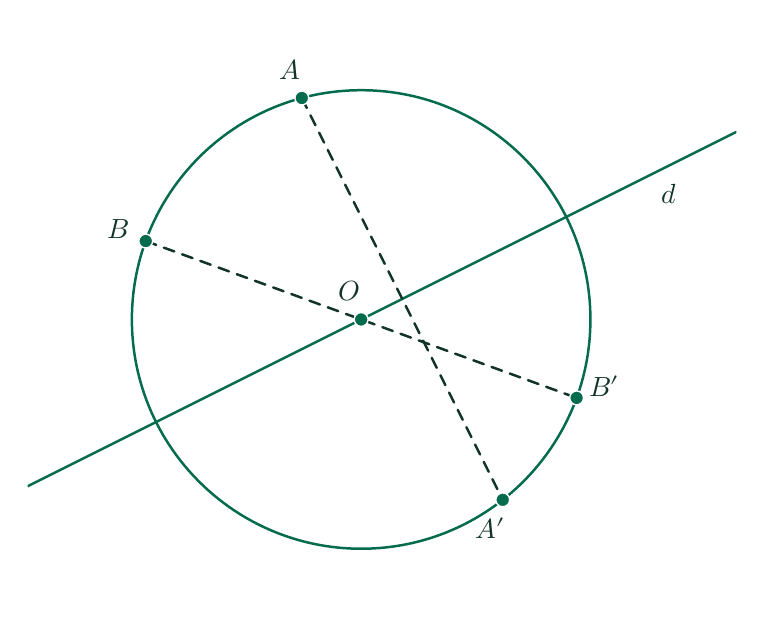
\begin{tikzpicture}[x=1.3235cm, y=1.3235cm]
\tkzDefPoint(0,0){O}
\tkzDefPoint(-0.5694,2.125){A}
\tkzDefPoint(1.3584,-1.7305){A1}
\tkzDefPoint(-2.0673,0.7524){B}
\tkzDefPoint(2.0673,-0.7524){B1}
\tkzDefPoint(2.2,0){tmp1}
\tkzDefPoint(3.6,1.8){tmp2}
\tkzDefPoint(-3.2,-1.6){tmp3}
\begin{scope}
\clip (-3.2,-2.8) rectangle (3.6,2.8);
\tkzDrawCircle[draw={rgb,255:red,4;green,107;blue,77}, line width=0.9pt](O,tmp1)
\tkzDrawSegment[draw={rgb,255:red,4;green,107;blue,77}, line width=0.90pt](tmp2,tmp3)
\tkzDrawSegment[draw=ink, line width=0.90pt, dash pattern=on 4pt off 3pt](A,A1)
\tkzDrawSegment[draw=ink, line width=0.90pt, dash pattern=on 4pt off 3pt](B,B1)
\end{scope}
\node[dot, fill={rgb,255:red,4;green,107;blue,77}] at (O) {};
\node[dot, fill={rgb,255:red,4;green,107;blue,77}] at (A) {};
\node[dot, fill={rgb,255:red,4;green,107;blue,77}] at (A1) {};
\node[dot, fill={rgb,255:red,4;green,107;blue,77}] at (B) {};
\node[dot, fill={rgb,255:red,4;green,107;blue,77}] at (B1) {};
\node[lab, font=\normalsize] at (2.95,1.2) {$d$};
\node[lab, font=\normalsize, anchor=center, xshift=-4.21pt, yshift=10.16pt] at (0,0) {$O$};
\node[lab, font=\normalsize, anchor=center, xshift=-4.21pt, yshift=10.16pt] at (-0.5694,2.125) {$A$};
\node[lab, font=\normalsize, anchor=center, xshift=-4.21pt, yshift=-10.16pt] at (1.3584,-1.7305) {$A'$};
\node[lab, font=\normalsize, anchor=center, xshift=-10.16pt, yshift=4.21pt] at (-2.0673,0.7524) {$B$};
\node[lab, font=\normalsize, anchor=center, xshift=10.16pt, yshift=4.21pt] at (2.0673,-0.7524) {$B'$};
\end{tikzpicture}
\end{document}
